\section{Partial Wave Analysis II}
\subsection{Review of Last Class}
We developed partial wave analysis as a tool to study scattering problems in a more general setting. The only information that enters is the phases/partial wave amplitudes:
\begin{equation}
    f_l = \frac{S_l - 1}{2ik} = \frac{e^{i\delta_l}\sin(\delta_l)}{k}
\end{equation}
we derived this, and our cross section is expressed explicitly in terms of these partial wave amplitudes:
\begin{equation}
    f(\theta) = \sum_l f_l P_l(\cos\theta)(2l+1)
\end{equation}
where $P_l$ gives the angular distribution (we neglect the $\phi$ dependence from symmetry) and the $2l+1$ comes from the degeneracy.

\subsection{Complex Structure of Partial Wave Amplitudes}
Let us look at the complex structure of the partial wave amplitudes - this will be an important lead-in for our discussion on resonance scattering. Taking the imaginary part, we have:
\begin{equation}
    \text{Im}f_l = \frac{\sin^2(\delta_l)}{k} = \frac{k^2\abs{f_l}^2}{k} = k\abs{f_l}^2
\end{equation}
which might be familiar as the Optical theorem (here applied to partial wave amplitudes). Looking at the imaginary part of the inverse partial wave amplitude, we have:
\begin{equation}
    \text{Im}\frac{1}{f_l} = \text{Im}\frac{f_l^*}{\abs{f_l}^2} = -k
\end{equation}
and so:
\begin{equation}\label{eq-fl}
    \frac{1}{f_l} = g_l(k) - ik
\end{equation}
where $g_l$ is the real part. This is an extremely generic formula. It has far-reaching physical signficance, which we shall get to soon.

\subsection{Example - Attractive Potential}
We consider $U = -U_0$ for $r \leq a$, and $k^2 = \frac{2mE}{\hbar^2}$ as usual.

\begin{figure}[htbp]
    \centering
    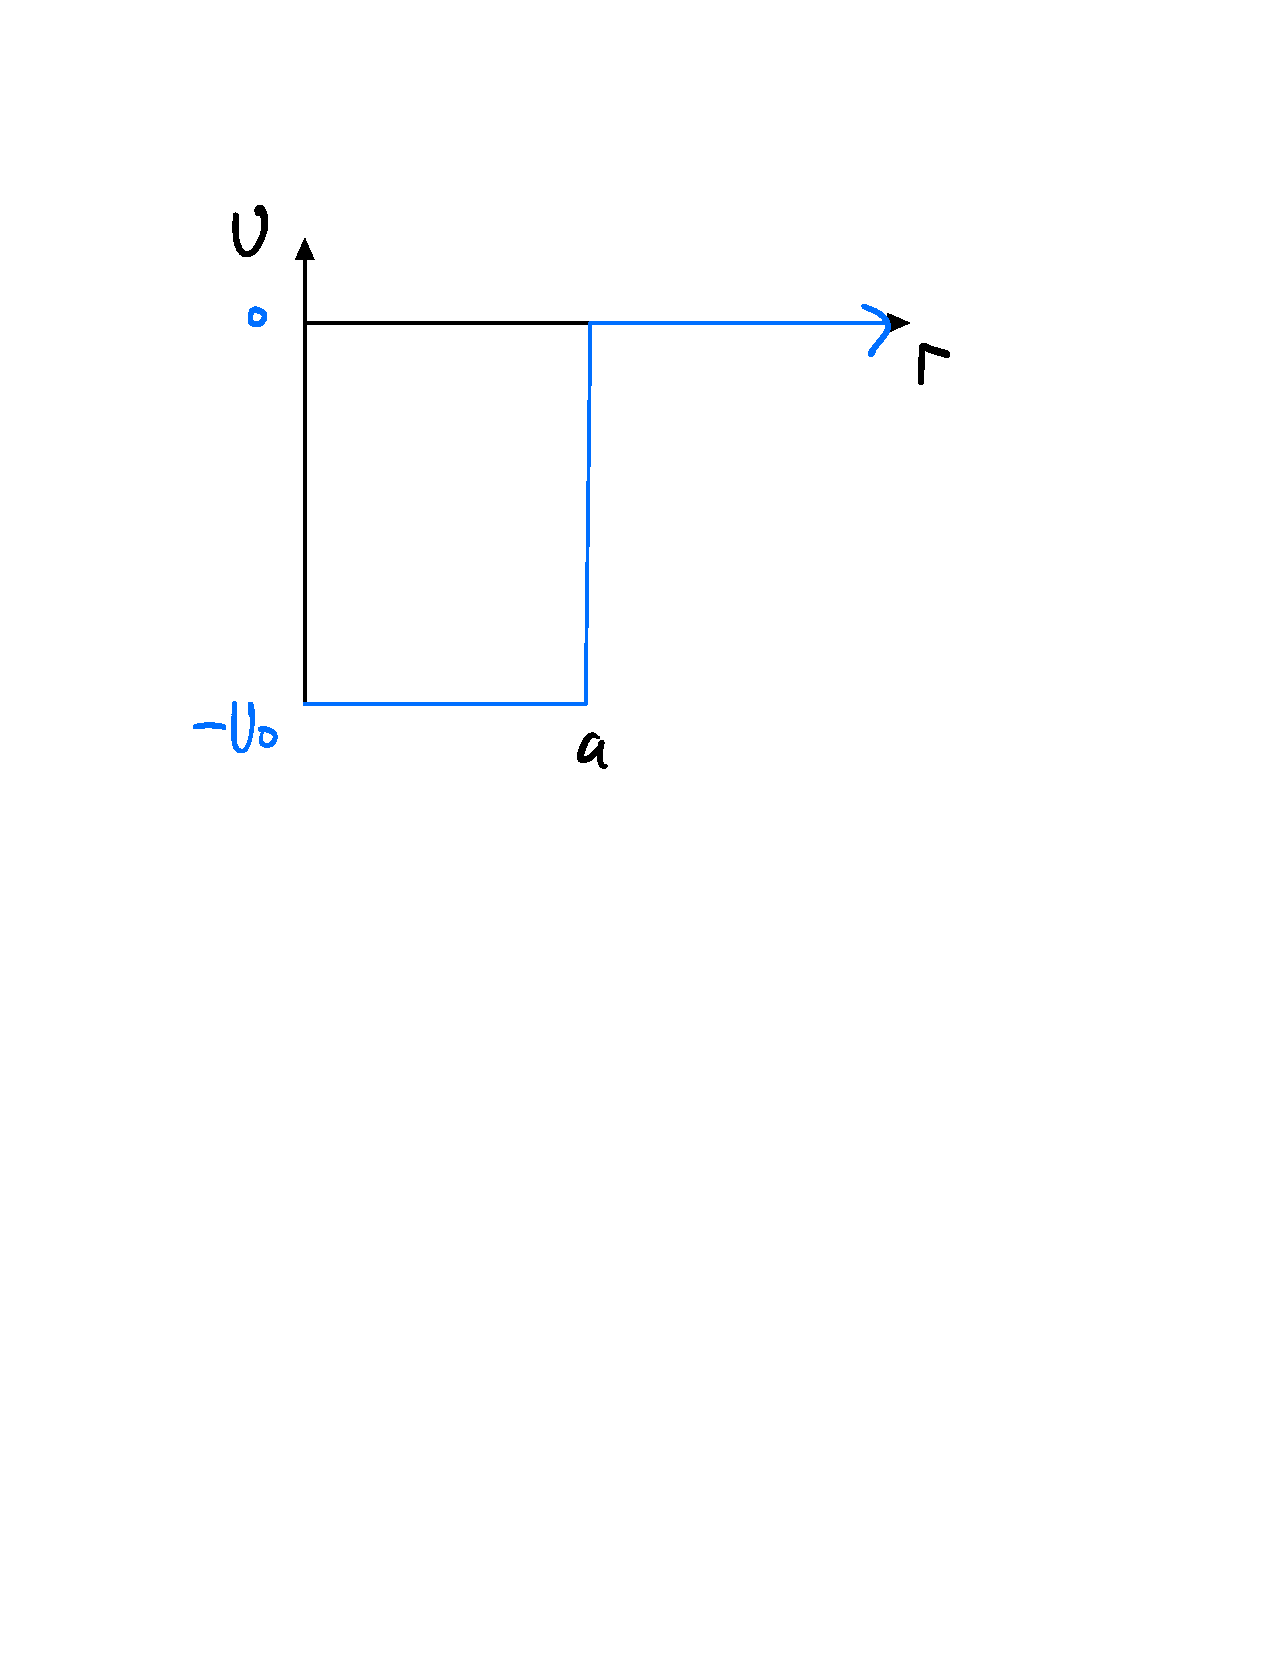
\includegraphics[scale=0.6]{Images/fig-squarewell.pdf}
    \caption{Attractive radial square well potential which we analyze via partial wave analysis.}
    \label{fig-squarewell}
\end{figure}

We then have the conventional normalization:
\begin{equation}
    \int r^2 dr R_{kl}(r)R_{k'l'}(r) = \delta_{ll'}\delta_{kk'}
\end{equation}
(or replace $\delta_{kk'} \to \delta(k-k')$ if the $k$s are continuous). We then right down the radial SE as:
\begin{equation}
    R_{kl}'' + \frac{2}{r}R_{kl} + \left(k^2 + \frac{l(l+1)}{r^2}\right)R_{kl} = 0
\end{equation}

Let us solve this problem in the very simple case of $l = 0$. We do the very convenient change of variables $u = rR(r)$, which yields:
\begin{equation}
    u'' + k^2 u = 0, \quad r \geq a
\end{equation}
\begin{equation}
    u'' + \chi^2 u = 0, \quad r \leq a
\end{equation}
where $\chi^2 = \frac{2m(E + \abs{U_0})}{\hbar^2}$. 

For $r \leq a$, we have $u = A\sin(\chi r)$ (the cosine term vanishes). For $r \geq a$, we have $u = B\sin(kr - \delta_0)$. In principle, we can have a cosine and sine term, but we instead introduce a phase factor in a very precise way, as:
\begin{equation}
    R_{kl}(r \to \infty) = \frac{\sin(kr - \frac{l\pi}{2} + \delta_l)}{r}
\end{equation}
Now, we write:
\begin{equation}
    S_l \frac{e^{ikr}}{r} = e^{2i\delta_l}\frac{e^{ikr}}{r}
\end{equation}
So if we are able to calculate the phase factor, we therefore can determine everything about the structure of the problem. How we do the analysis is as follows. We consider:
\begin{equation}
    \left. \frac{u'}{u}\right|_{r \leq a} = \left. \frac{u'}{u}\right|_{r \geq a}
\end{equation}
which follows from the continuity of the wavefunction and at the derivative at $r = a$. We then find:
\begin{equation}
    \chi \frac{\cos(\chi a)}{\sin(\chi a)} = k\frac{\cos(ka + \delta_0)}{\sin(ka + \delta_0)}
\end{equation}
Now, we discuss solutions $\delta$ to this equation. Note that we consider $\chi$ finite here (and will deal with the special case of otherwise later).

First, we suppose the case of low-energy scattering, where $k \to 0$. The solution is very simple. We see precisely that in order to have nontrivial solutions, our phase must be vanishing in order to have a nontrivial solution. The only way to get a finite number as $k \to 0$ is to have the phase vanishes with $k$, such that $\frac{k}{\sin(ka + \delta)}$ must be finite.


Mathematically, if we Taylor expand the RHS:
\begin{equation}
    k\cot(ka + \delta) = \frac{k}{ka + \delta(k)}
\end{equation}
Now, we go back to the original equation, and what we say is that:
\begin{equation}
    \chi\cot(\chi a) \approx \frac{k}{ka + \delta(k)}
\end{equation}
and so:
\begin{equation}
    ka + \delta = \frac{k}{\chi\cot(\chi a)}
\end{equation}
so:
\begin{equation}
    \delta = \frac{k}{\chi\cot(\chi a)} - ka = ka\left(\frac{\tan(\chi a)}{\chi a} - 1\right)
\end{equation}
so $\delta \to 0$ as $k \to 0$. 

Knowing the phase, the amplitude computation is trivial:
\begin{equation}
    f = \frac{e^{2i\delta_0} - 1}{2ik} \approx \frac{1 + 2i\delta_0 - 1}{2ik} = \frac{\delta_0}{k} = a\left(\frac{\tan \chi a}{\chi a} - 1\right)
\end{equation}
and so:
\begin{equation}
    \sigma = \int d\sigma = \int \abs{f}^2 d\Omega = 4\pi a^2 \left(\frac{\tan \chi a}{\chi a} - 1\right)^2
\end{equation}
Note that in PT $U_0$ was small. But now, we are able to do computations for arbitrarily large potentials.

We can immediately see for large $U_0$ that:
\begin{equation}
    \sigma \to 4\pi a^2.
\end{equation}
this is the famous result when $U_0 \to \infty$, $k \to 0$. Compare to the classical mechanics result when $\sigma = \pi a^2$. Where does the extra factor of $4$ come from? It comes from QM (of course). When $k \to 0$, it follows that $\lambda \gg a$. So, he scattering is not just happening from one surface of the hard sphere, but from every direction - so we can have scattering from any part of the sphere!

\begin{figure}[htbp]
    \centering
    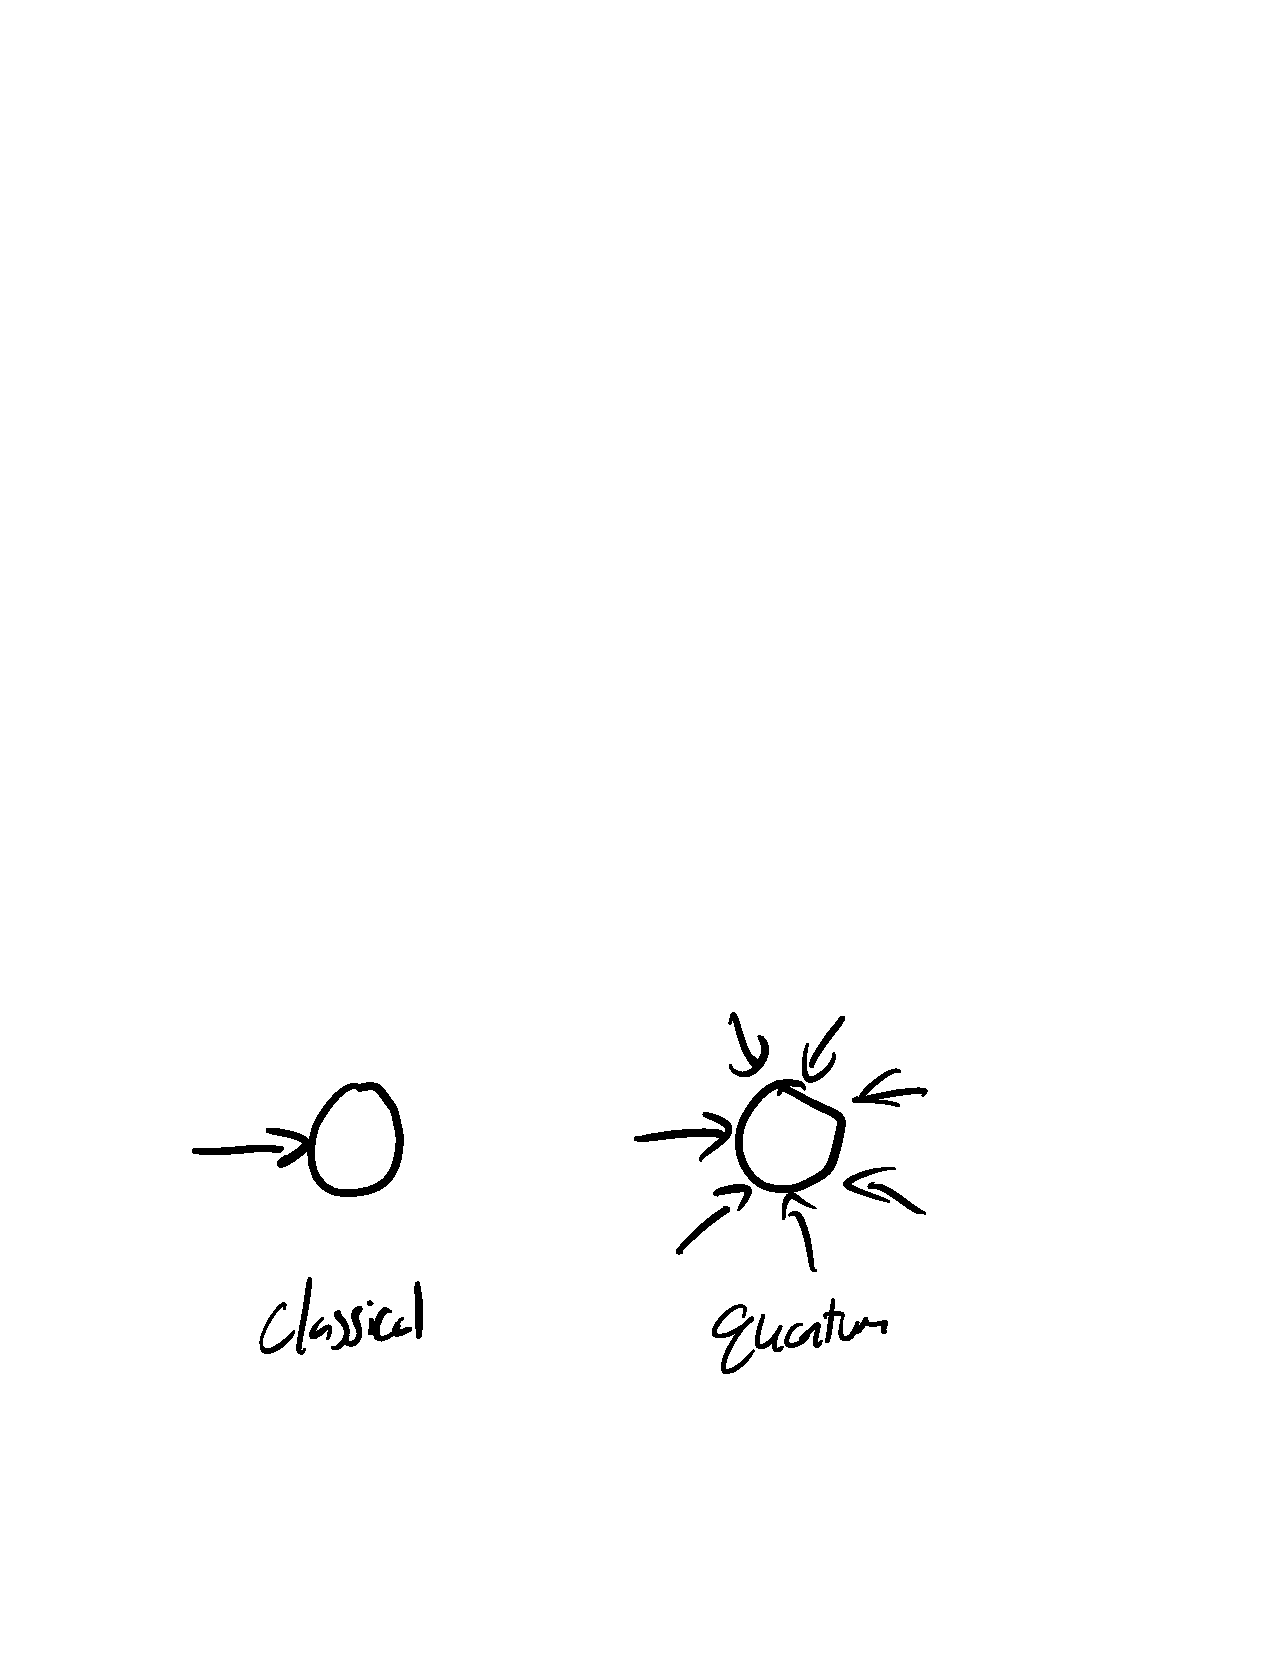
\includegraphics[scale=0.5]{Images/fig-quantumhardsphere.pdf}
    \caption{Low-energy hard sphere scattering in the classical (where the direction of scattering is limited, so $\sigma = \pi a^2$) and quantum (where the particle can scatter off of any part of the sphere, yielding $\sigma = 4\pi a^2$) cases.}
    \label{fig-quantumhardsphere}
\end{figure}

\subsection{Reproducing the PT contribution}
For small potentials $U_0$, we should recover the perturbation theory/Born approximation result. Let us therefore expand:
\begin{equation}
    \tan(\chi a) = \frac{\sin(\chi a)}{\cos(\chi a)} \approx \frac{\chi a (1 - \frac{(\chi a)^3}{3!})}{(1 - \frac{(\chi a)^2}{2!})} = \chi a \left(1 + \frac{1}{3}(\chi a)^2\right)
\end{equation}
so:
\begin{equation}
    \sigma = 4\pi a^2\left(\frac{\tan \chi a}{\chi a} - 1\right)^2 \approx 4\pi a^2 \frac{1}{9}(\chi a)^2
\end{equation}
which is the result for the case for small potential and small energies.

In the Born approximation, we have:
\begin{equation}
    f = \frac{m}{2\pi \hbar^2}U_0 \frac{4}{3}\pi a^4 = \frac{mU_0}{\hbar^2}\left(\frac{2}{3}a^3\right)
\end{equation}
so then using that $a^2\chi^2 = \frac{2mU_0 a^2}{\hbar^3}$:
\begin{equation}
    f = \frac{\chi^2 a}{3}a
\end{equation}
so the two methods agree in the low-potential limit. However, the formula obtained by the partial wave analysis is more general.

\subsection{Resonance Scattering}
Let us return to our solution:
\begin{equation}
    \chi \cot(\chi a) = k \cot(ka + \delta)
\end{equation}
where $\delta$ does \emph{not} go to zero. However, we still consider the low energy case where $ka \to 0$. Solutions can actually exist here, in the form $\delta \to \frac{\pi}{2} + \pi n$.

We write:
\begin{equation}\label{eq-tandelta}
    \tan \delta = \frac{k}{\chi}\tan(\chi a), \quad k \to 0
\end{equation}
Let us represent the amplitude in the following way:
\begin{equation}
    f = \frac{e^{i\delta}\sin\delta}{k} = \frac{\sin \delta}{k(\cos \delta - i \sin \delta)} = \frac{1}{k(\cot \delta - i)} = \frac{1}{k\cot \delta - ik}
\end{equation}
Now, we apply: Eq. \eqref{eq-tandelta}.
\begin{equation}
    f = \frac{1}{\chi \cot(\chi a) - ik}
\end{equation}

Now, recall that in the most generic form, $f_l = \frac{1}{g_l - ik}$ (from Eq. \eqref{eq-fl}). then, notice that $f \to \frac{1}{-ik}$ if $\cot \chi a \to 0$. This is unbelievable; the cross section whichis $\sigma = 4\pi \abs{f}^2 \to \frac{4\pi}{k^2}$ But then as $k \to 0$, $\sigma \to \infty$!!! The cross section becomes infinitely large - much larger than the size of the system! How could this possibly happen? For an infinitely attractive potential we found $4\pi a^2$, which one might naively think is the maximum possible, but no actually, it could be infinite large! In classical physics this is impossible. It is due to a resonance - think about why this could lead to such a cross section.

We quote a general result:
\begin{equation}
    \sigma = 4\pi \abs{f}^2 = \frac{4\pi a^2}{\left(\left(\chi a\cot(\chi a)\right)^2 + k^2a^2\right)}
\end{equation}
The idea is that the total-cross section can be arbitrarily large, and in order to understand why this happens, we have ot understand what is happening with the $\chi a \cot \chi a$ term. We will want to explicitly solve the problem of the energy being slightly negative. We are very close to understanding what is going on here, and we will explore it in the next lecture.

